\documentclass[10]{article}
\usepackage[titletoc, title]{appendix}
\usepackage{graphicx}
\usepackage{pdfpages}
\usepackage{float}
\usepackage{gensymb}
\usepackage{subfig}

%opening
\title{Software Design Document}
\author{Michael Farghali}

\begin{document}

\maketitle


\section{Introduction}
This Software Design Document (SSD) will give a very high overview of my Pascal complier which is based on the grammar rules given at the start of the course. The goal of this keystone course was to write a compiler in Java that accepts a text file representing a reduced version of Pascal. The text file will be scanned, parsed, converted into a syntax tree and finally written to an output file in assembly language. Upon completion of the course an executable .jar file should be submitted that does the above along with a user manual that explains how to run the program and any possible error messages. 
 
\section{Scanner}

The purpose of the scanner class is to read in the source code and match all valid keywords and IDs with their respective TokenType which are in the LookupTable class. It is based on a Deterministic Finite Automaton, Fig. \ref{fig: fg1}, and the given grammars seen in appendix \ref{grammars}. Each state in the DFA represents a state in the scanner. 
\begin{figure}[!ht]
	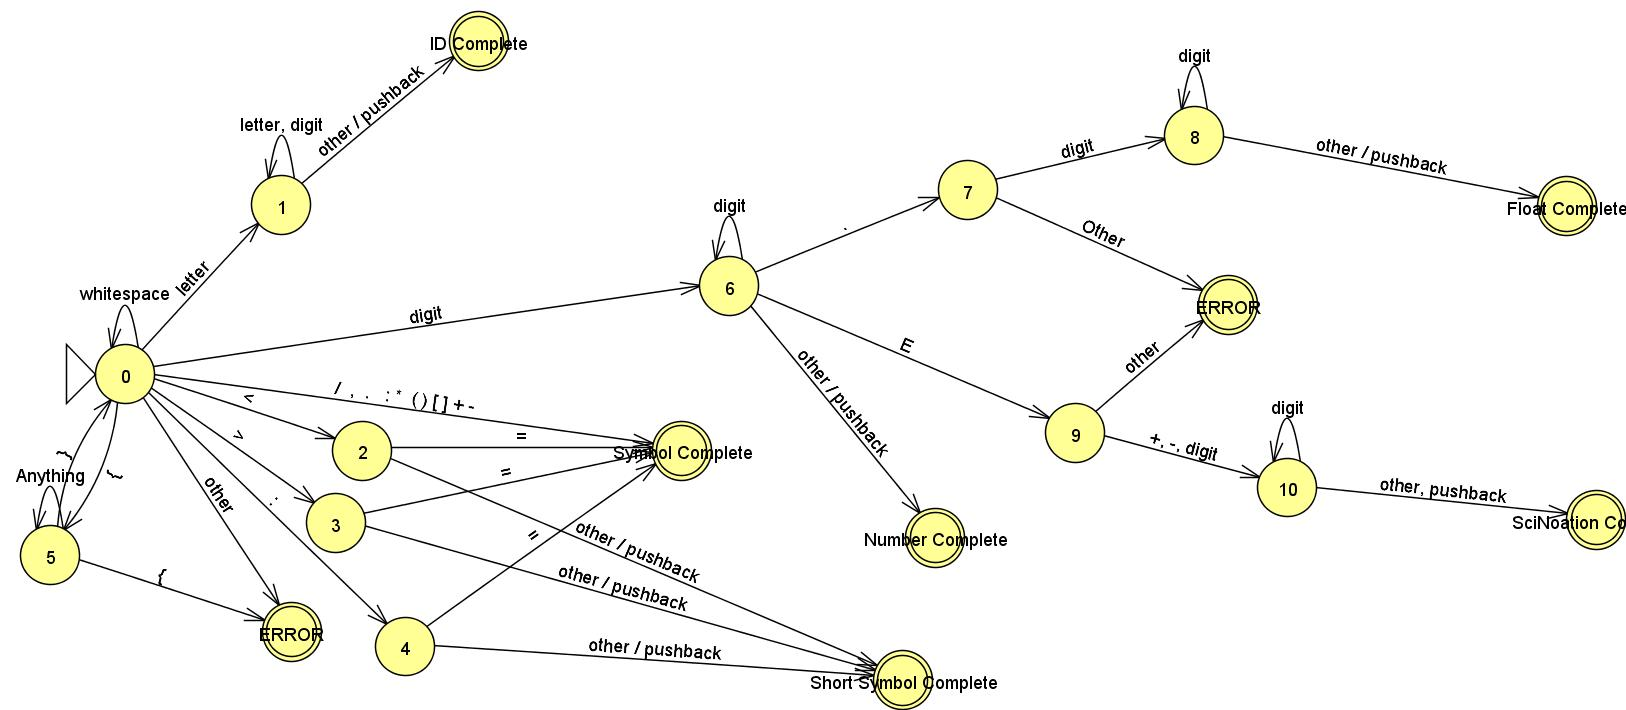
\includegraphics[width=\textwidth]{ScannerDFA.jpg}
	\caption{DFA \label{fig: fg1}}
	
\end{figure}

The scanner passes information to the Parser class primarily through the methods \verb|nextToken|, \verb|getToken|, and \verb|getLexeme|. Most of the work done in the scanner class is done in the nextToken method which is responsible for checking that keywords are valid in our language and that IDs are also in a format allowed and returns true is so or false if not. The getToken method will be used by the parser to grab the current token from the scanner. Finally the getLexeme method is used to pass the name of a variable or invalid statement in the source code, to the parser. 

\paragraph{}
I chose to deviate from the example given in class and added methods \verb|pushBackChar| and \verb|getNextChar|. These methods don't do anything new but the code is used multiple times in the scanner class so I decided to create their own functions to clean up the nextToken method. I also added a method \verb|getCount()| which simply returns the line number where the scanner encounters an unexpected or invalid string. The UML for the scanner class can be seen below.

\begin{figure}[!ht]
	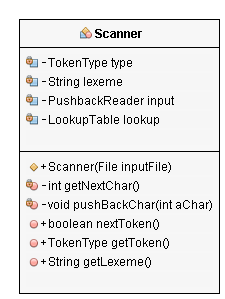
\includegraphics[height=3in]{ScannerUML.png}
	\caption{Scanner \label{fig: fg2}}
\end{figure}

\subsection{Testing}
To test the scanner I created a JUnit test that tested all the methods focusing mainly on the \verb|nextToken| method. I tested it using several valid and invalid strings. Some examples 

\section{Parser}

The Parser class is responsible for a large portion of the work being done in this compiler. It uses the Context-Free grammar rules listed in Appendix \ref{grammars} and a push down automata to either accept or reject a source file. It uses top down recursive decent parsing which is convenient for implementation as all 24 nonterminal rules in our grammar become methods in the code. The UML diagram can be seen in \ref{fig: fg3}.
\begin{figure}[!ht]
	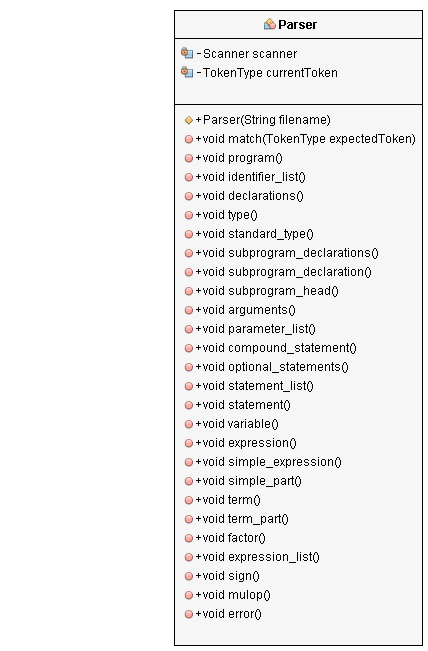
\includegraphics[height=4in]{ParserUML.png}
	\caption{Parser UML \label{fig: fg3}}
\end{figure}

\paragraph{}
In the parser I chose not to follow the grammar rules exactly. I added methods \verb|addop| and \verb|mulop| which determine which kind of arithmetic or multiplication operator is being used. Adding these two functions helped to clean up the code and make it more readable in my opinion. I also deleted two methods, \verb|simple_part| and \verb|term_part| and added their functionality to \verb|simple_expression| and \verb|term|. To me this seems more straightforward and easy to follow.

\paragraph{}
The parser class communicates with the Scanner, Symbol Table, and all the classes in Syntax Tree. It uses the scanner to get tokens and the name or string that the token represents. The symbol table is built up and printed to a file in the parser. The parser also creates a condensed syntax tree and if there is an error in the syntax this is where it should be caught. 

\subsection{Testing}
The parser was tested with multiple files containing both valid and invalid code. It tested for simple programming errors such as a missing semicolon as well as syntax error.  

\subsection{Semantic Analysis}
In the semantic analysis stage of the complier three errors should be handled without ending the compilation process. First, variables and assignments should be assigned their data type so that variables of type real can be assigned integer values but not the other way around. There should also be a check that variables are declared before being used. Finally, the syntax tree should print out the variable or expression's type.

\paragraph{}
We were given the option of implementing the semantic analysis code in the parser or in a separate module. I chose to include it in the parser by adding the function \verb|undeclaredVarError| to handle undeclared variables. To add the variable and expression type to the symbol table I was only able to add their type at declaration time. 


\section{Symbol Table}
The Symbol Table class implements a hashtable and data structure to keep track of variables, functions, procedures, and the program ID. It should also handle arrays and their index. By integrating the symbol table into the parser it is possible for the parser to do the semantic analysis by checking if an ID is in the table. I implemented my symbol table by creating a separate method to add each kind of ID, program, array, function, procedure, and variable. I also created a method to check if each type is already in the table thus allowing the parser to check if the same ID is being used more than once in the same scope. The symbol table should also be used in the parser to handle function and variable scope. The UML diagram can be seen in Fig. \ref{fig: fg4}.


\begin{figure}[!thp]
	\centering
	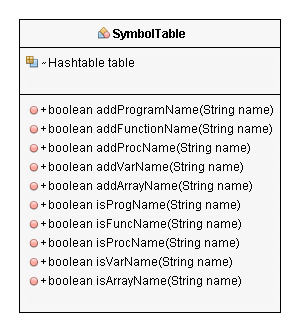
\includegraphics[width=3in, height=3in]{SymTableUML.png}
	\caption{SymbolTable UML \label{fig: fg4}}
\end{figure}

\subsection{Testing}
Testing the symbol table was a simple task. I checked that the same ID couldn't be added to the table if it already existed and also checked that if it already existed in the table it would return true.

\section{Syntax Tree}
The syntax tree package contains 14 classes that represent the different statements, variables, and operations in our Pascal. Each class (node) is responsible for adding it's part of the tree to the syntax tree which will be used by the code generation part of the compiler. The UML diagrams for the multiple classed can be seen in appendix C.

\subsection{Testing}
Testing the syntax tree was straightforward but tedious. I created a JUnit test and manually built a properly formated syntax tree for our bitcoins sample program. I then ran the complier against the sample code verifying that the two matched. 



\section{Code Generator}
The final task of the compiler was of course to produce some MIPS assembly code. A new class, CodeGeneration, was used to write all the assembly code to a file named after the program. The code generator creates assembly code similar to the way the parser created a syntax tree. 

\subsection{Testing}
To test the code generation I used QTSpim and manually stepped through the code seeing that the registers were being assigned the proper value. 

\begin{figure}[!ht]
	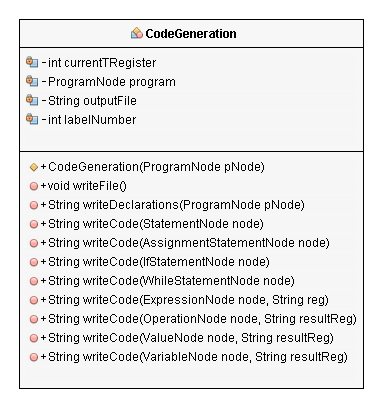
\includegraphics[height=4in]{CodeGen.png}
	\caption{CodeGeneration UML }
\end{figure}


\newpage
\begin{appendices}

\section{List of Keywords}
\label{keywords}
Symbols: $ . , - + * / ( ) { } [ ] { } < <= > >= : := ;$  
\newline
Keywords: div, mod, and, program, id, var, array, of, num, integer, real, function, procedure, begin, end, if, then, else, while, do, not

\section{Grammar Rules}
\label{grammars}
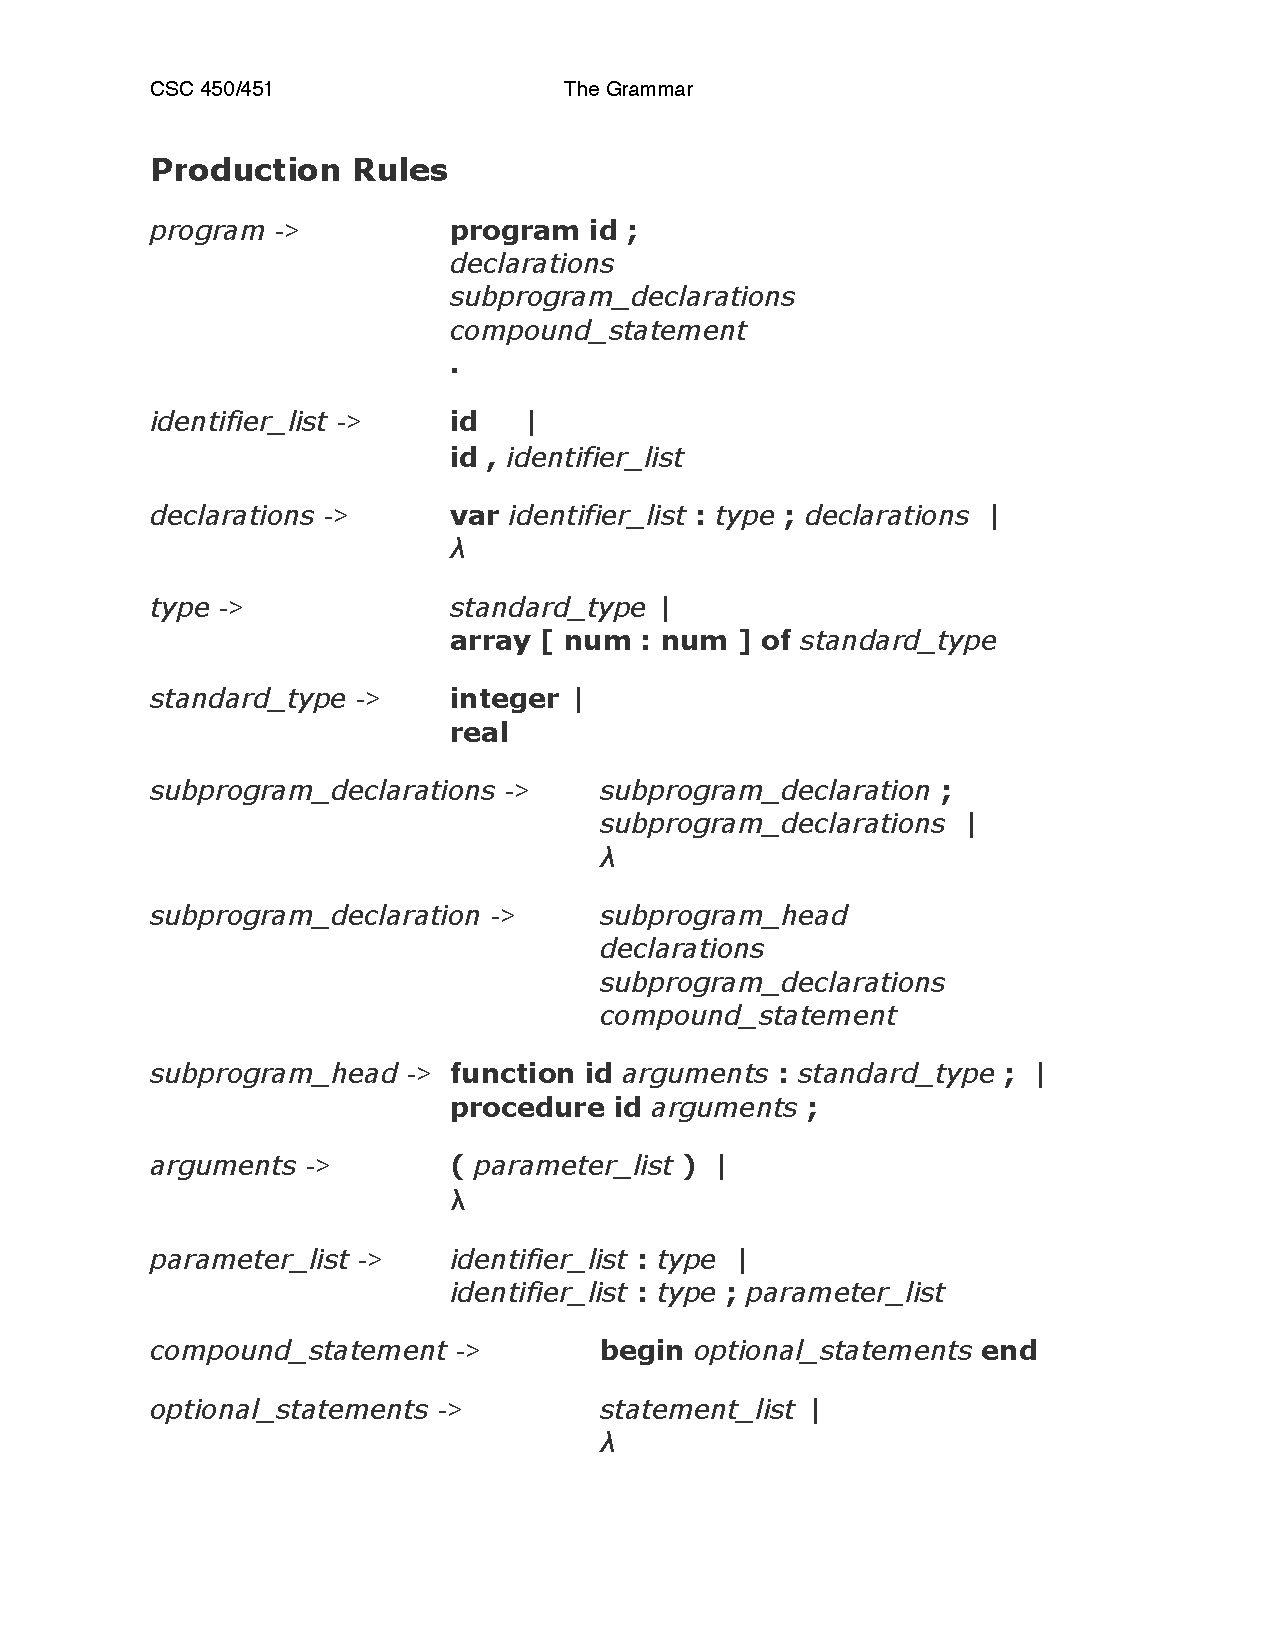
\includepdf[pages=-, scale=.8, noautoscale = true]{Grammar.pdf}

\section{Syntax Tree UML}
\begin{figure}[!thp]
	\centering
	\subfloat[]{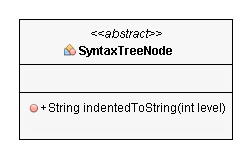
\includegraphics[width=0.4\textwidth]{syntaxtree.png}}
	\hfill
	\subfloat[]{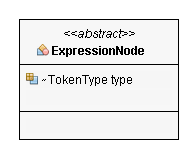
\includegraphics[width=0.4\textwidth]{expression.png}}
\end{figure}

\begin{figure}[!thp]
	\centering
	\subfloat[]{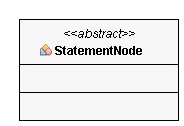
\includegraphics[width=0.4\textwidth]{statement.png}}
	\hfill
	\subfloat[]{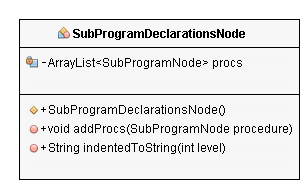
\includegraphics[width=0.4\textwidth]{subprogramdeclarations.png}}
	\caption{}
\end{figure}

\begin{figure}[!thp]
	\centering
	\subfloat[]{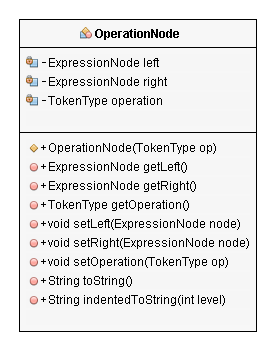
\includegraphics[width=0.4\textwidth]{operation.png}}
	\hfill
	\subfloat[]{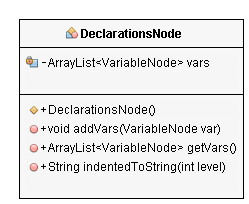
\includegraphics[width=0.4\textwidth]{declarations.png}}
	\caption{}
\end{figure}

\begin{figure}[!thp]
	\centering
	\subfloat[]{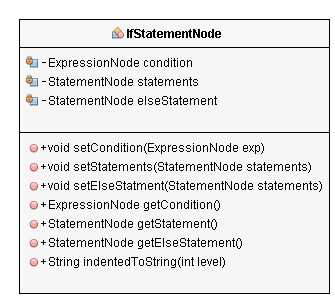
\includegraphics[width=0.4\textwidth]{ifstatement.png}}
	\hfill
	\subfloat[]{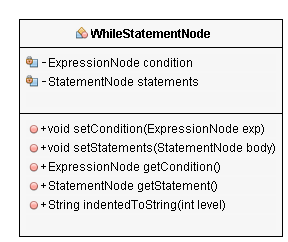
\includegraphics[width=0.4\textwidth]{while.png}}
	\caption{}
\end{figure}

\begin{figure}[!thp]
	\centering
	\subfloat[]{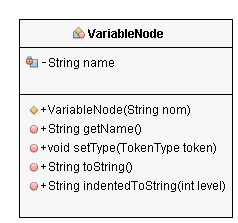
\includegraphics[width=0.4\textwidth]{variable.png}}
	\hfill
	\subfloat[]{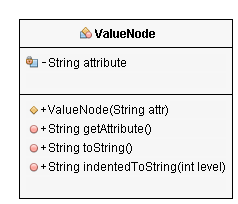
\includegraphics[width=0.4\textwidth]{value.png}}
	\caption{}
\end{figure}

\end{appendices}

\end{document}
